\section[Propriétés utiles de l'algèbre linéaire]{Propriétés utiles de l'algèbre linéaire}

\begin{frame}{Propriétés utiles de l'algèbre linéaire}
	Dans cette section, nous exploiterons certaines propriétés très utiles de l'algèbre linéaire à la fois pour:
	\begin{itemize}
		\item \textbf{déterminer} les composantes principales, 
		\item \textbf{interpréter} les résultats d'un point de vue \textit{géométrique} et \textit{statistique},
		\item \textbf{simplifier} le problème d'apprentissage statistique par un changement de base \textit{partiel} des caractéristiques d'entrée $X$.
	\end{itemize}
\end{frame}

\subsection[Matrice de covariance]{Matrice de covariance}

\begin{frame}{Particularité de la matrice de covariance}
	\begin{itemize}
		\item La matrice de covariance des colonnes de $X$ notée $\Sigma \in \mathcal{M}_{p,p}(\R)$ est une matrice \textbf{carrée} et \textbf{symétrique} par construction et grâce à la symétrie de l'opérateur covariance.
		\pause
		\item Elle est également \textbf{semi-définie positive}. Pour tout vecteur $v \in \mathcal{M}_{p,1}(\R)$ on pourrait montrer que $v^T \Sigma v \ge 0$.
		\pause
		\item \'Etant symétrique, les vecteurs propres $u$ sont \textbf{orthogonaux} entre eux et les valeurs propres sont \textbf{réelles}.
		\pause
		\item De plus, étant semi-définie positive, les valeurs propres $\lambda$ sont nécessairement \textbf{positives ou nulles}.
	\end{itemize}
\end{frame}

\begin{frame}{Décomposition spectrale de la matrice de covariance}
	La décomposition spectrale de la matrice de covariance est donnée par:
	\begin{equation}
		\Sigma = U \Lambda U^T
		\nonumber
	\end{equation}
	Avec $U \in \mathcal{M}_{p,p}(\R)$ la matrice orthogonale ($U^T U = I_p$ ou encore $U^T = U^{-1}$) constituée des vecteurs propres:
	\begin{equation}
		U = \begin{pmatrix}
			\vert & \vert & \cdots & \vert \\
			u_1   & u_2   & \cdots & u_p   \\
			\vert & \vert & \cdots & \vert
		\end{pmatrix}
		\nonumber
	\end{equation}
	Et $\Lambda \in \mathcal{M}_{p,p}(\R)$ une matrice diagonale constituée des valeurs propres:
	\begin{equation}
		\Lambda = \begin{pmatrix}
			\lambda_1 & 0 & \cdots & 0 \\
			0 & \lambda_2 & \cdots & 0 \\
			\vdots & \vdots & \vdots & \vdots \\
			0 & 0 & \cdots & \lambda_p
		\end{pmatrix} \quad \text{avec} \quad \lambda_1 \ge \lambda_2 \ge \dots \ge \lambda_p
		\nonumber
	\end{equation}
\end{frame}

\begin{frame}{Représentation graphique}
	\begin{columns}
		\begin{column}{0.5\textwidth}
			\begin{figure}
				\centering
				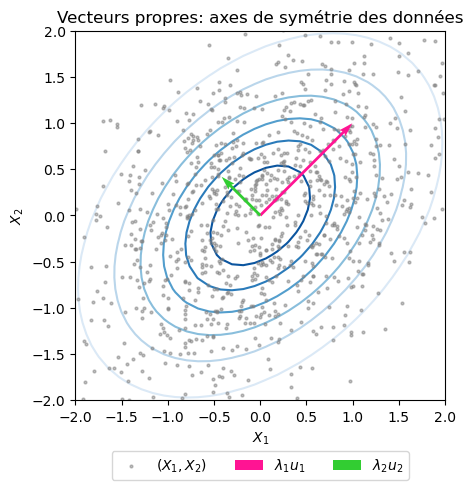
\includegraphics[height=1.0\linewidth]{Images/axes_de_symétrie}
				\label{fig:axes_de_symétrie}
			\end{figure}			
		\end{column}
		\begin{column}{0.5\textwidth}
			Dans la figure ci-contre, dans un espace $\R^2$ on voit les iso-probabilités idéalisées représentatives de la matrice de covariance. Le vecteur propre de la première composante principale est aligné avec le grand axe, alors que le vecteur propre de la seconde composante principale est aligné avec le petit axe. Les valeurs propres représentent la longueur des axes des ellipses.
		\end{column}
	\end{columns}
\end{frame}

\begin{frame}{Changement de base}
	La matrice $U$ est la matrice de passage de la base $\mathcal{B}$ associée à l'espace des caractéristiques d'entrée $\mathcal{X}$ à une nouvelle base $\mathcal{B}^{'}$ dans laquelle la matrice de covariance est diagonale. La matrice $U^T$ est la matrice de passage inverse, de $\mathcal{B}^{'}$ dans $\mathcal{B}$:
	\begin{equation}
		\Lambda = U^T \Sigma U
		\nonumber
	\end{equation}
	Dans la base $\mathcal{B}^{'}$, les caractéristiques d'entrée n'ont plus d'inter-dépendance (elles sont complètement décorrélées).
\end{frame}

\begin{frame}{Changement de base}
	Le changement de base de $\mathcal{B}$ à $\mathcal{B}^{'}$ pour les observations des caractéristiques d'entrée $X$ s'écrit:
	\begin{equation}
		Z = X U
		\nonumber
	\end{equation}
	Le score $Z \in \mathcal{M}_{n,p}(\R)$ intègre désormais l'ensemble des $p$ composantes principales.
\end{frame}

\begin{frame}{Changement de base}
	Voici un exemple de changement de base en utilisant tous les vecteurs propres quand un espace des caractéristiques d'entrée est $\R^2$:
	\begin{figure}
		\centering
		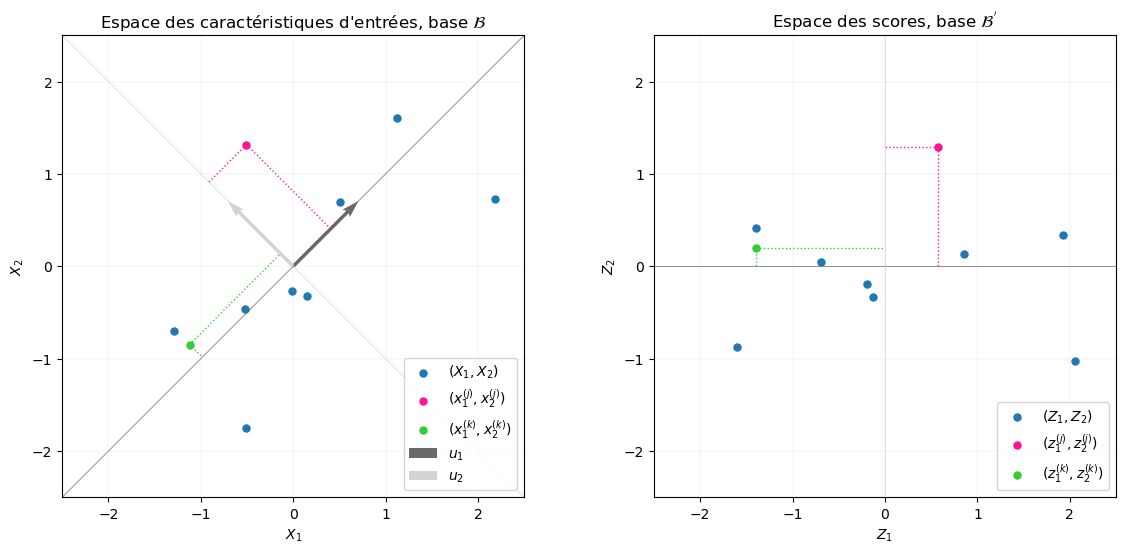
\includegraphics[width=0.95\linewidth]{Images/changement_de_base}
		\label{fig:changement_de_base}
	\end{figure}
\end{frame}

\subsection[Détermination des valeurs et vecteurs propres]{Détermination des valeurs et vecteurs propres}

\begin{frame}{Définition des valeurs et vecteurs propres}
	Une matrice symétrique $\Sigma \in \mathcal{M}_{p,p}(\R)$ admet pour valeur propre un scalaire $\lambda \in \R$ et pour vecteur propre associé un vecteur $u \in \mathcal{M}_{p,1}(\R)$ non nul si et seulement si:
	\begin{equation}
		\Sigma u = \lambda u
		\nonumber
	\end{equation}
	La transformée de $u$ par $\Sigma$ est donc un vecteur colinéaire à $u$. \\
	\pause
	\vspace{0.5cm}
	Une écriture équivalente est:
	\begin{equation}
		\Sigma u - \lambda u = 0 \iff \left(\Sigma - \lambda I_p\right) u = 0
		\nonumber
	\end{equation}
	Or, comme on cherche $u$ comme un vecteur non nul et que le vecteur nul est une solution évidente au système d'équations linéaires précédent, il faut nécessairement que la matrice $\left(\Sigma - \lambda I_p\right)$ soit \textbf{singulière}.
\end{frame}

\begin{frame}{\'Equation caractéristique de la matrice $\Sigma$}
	Si la matrice $\left(\Sigma - \lambda I_p\right)$ est singulière, alors son déterminant doit être nul:
	\begin{equation}
		\det \left(\Sigma - \lambda I_p\right) = 0
		\nonumber
	\end{equation}
	Les solutions de cette \textbf{équation caractéristique}, non-linéaire en $\lambda$, donnent les valeurs propres de la matrice $\Sigma$.
\end{frame}

\begin{frame}{Représentation graphique}
	Dans un espace $\R^2$, les figures ci-dessous illustrent la transformation linéaire (endomorphisme) de l'espace opérée par une matrice symétrique. On voit que des points disposés sur les droites représentant les composantes principales restent sur ces mêmes droites en se rapprochant de l'origine (valeur propre plus petite que 1) ou en s'en éloignant (valeur propre plus grande que 1):
	\begin{columns}
		\begin{column}{0.5\textwidth}
			\begin{figure}
				\centering
				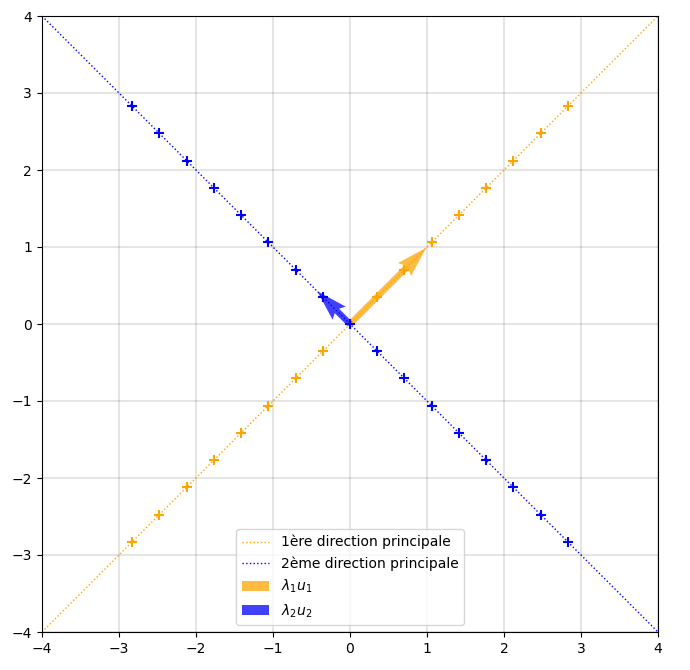
\includegraphics[height=0.85\linewidth]{Images/vecteur_valeur_propre_1}
				\label{fig:vecteur_valeur_propre_1}
			\end{figure}			
		\end{column}
		\begin{column}{0.5\textwidth}
			\begin{figure}
				\centering
				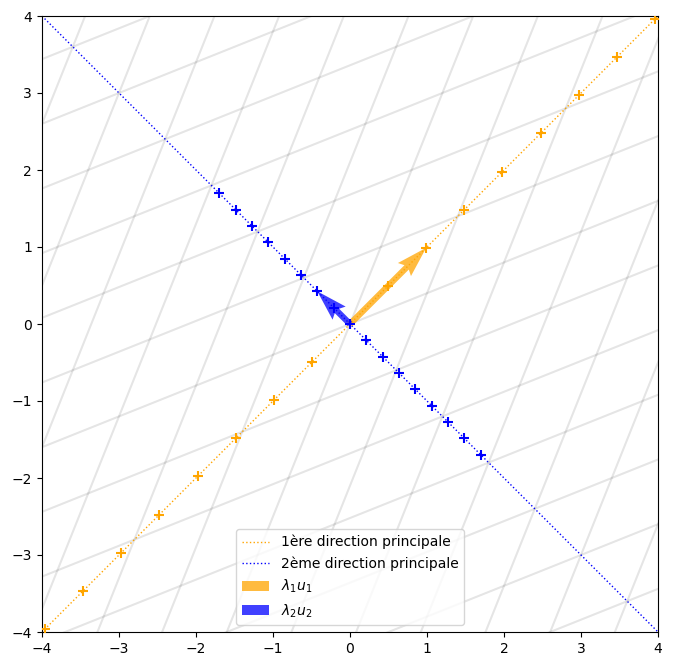
\includegraphics[height=0.85\linewidth]{Images/vecteur_valeur_propre_2}
				\label{fig:vecteur_valeur_propre_2}
			\end{figure}			
		\end{column}
	\end{columns}
\end{frame}

\subsection[Trace de la matrice de covariance]{Trace de la matrice de covariance}

\begin{frame}{Trace de la matrice de covariance}
	La trace de la matrice de covariance est la somme des termes diagonaux par définition. Donc:
	\begin{equation}
		\operatorname{Tr}(\Sigma) = \displaystyle \sum_{j=1}^p \Varhat{X_{\bigdot j}}
		\nonumber
	\end{equation}
	\pause
	La trace \textit{capture} donc la \textbf{totalité} de la variance des différentes caractéristiques d'entrée. Or une des propriétés de la trace d'une matrice, c'est qu'elle est \textbf{invariante au changement de base}. Par conséquent:
	\begin{equation}
		\operatorname{Tr}(\Sigma) = \displaystyle \sum_{j=1}^p \Varhat{X_{\bigdot j}} = \sum_{j=1}^p \lambda_j
		\nonumber
	\end{equation}
	Une interprétation de cette égalité est que la matrice $\Lambda$ a \textbf{complètement redistribué} la variance des caractéristiques d'entrée sur les valeurs propres, tout en éliminant les inter-dépendances.
\end{frame}

\begin{frame}{\'Eboulis de la variance et des valeurs propres}
	Une conséquence de cette propriété est qu'une valeur propre $\lambda_k$ représente à elle seule une fraction de la variance totale des colonnes de $X$:
	\begin{equation}
		\text{Ratio} = \frac{\lambda_k}{\sum_{j=1}^p \lambda_j}
		\nonumber 
	\end{equation}
	\pause
	Cette propriété est la clé de voûte de l'analyse en composantes principales:
	\begin{block}{Principe de simplification de l'ACP}
		La simplification repose sur la sélection des $k$-premières valeurs propres permettant de représenter une fraction \textit{suffisante} de la variance pour le problème d'apprentissage statistique.
	\end{block}
\end{frame}

\begin{frame}{Exemple de tracés d'éboulis des valeurs propres}
	\begin{columns}
		\begin{column}{0.5\textwidth}
			\begin{figure}
				\centering
				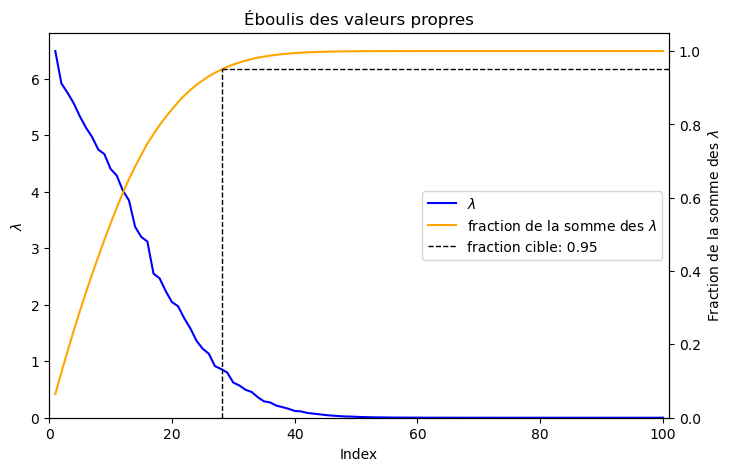
\includegraphics[width=1.0\linewidth]{Images/eboulis}
				\label{fig:eboulis}
			\end{figure}			
		\end{column}
		\begin{column}{0.5\textwidth}
			Dans le tracé ci-contre:
			\begin{itemize}
				\item On voit comment les valeurs propres décroissent de la première composante principale à la dernière.
				\item La courbe de fraction de la somme cumulée des $\lambda$, autrement dit, la fraction de variance expliquée, montre qu'en sélectionnant les 30 premières composantes principales, 95\% de la variance serait préservée.
			\end{itemize}
		\end{column}
	\end{columns}	
\end{frame}

\subsection[Réduction des dimensions]{Réduction des dimensions}

\begin{frame}{Simplification par calcul d'un score partiel}
	Le processus de simplification du problème consiste à sélectionner les $k \in \mathbb{N}$ plus grandes valeurs propres $\lambda_1, \lambda_2, \dots \lambda_k$ avec $k < p$ et leurs vecteurs propres associés $u_1, u_2, \dots u_k$ afin de calculer un score partiel $Z^* \in \mathcal{M}_{n,k}(\R)$:
	\begin{equation}
		Z^* = X U^*
		\nonumber
	\end{equation}
	Avec $U^* \in \mathcal{M}_{p,k}(\R)$ défini comme:
	\begin{equation}
		U^* = \begin{pmatrix}
			\vert & \vert & \cdots & \vert \\
			u_1   & u_2   & \cdots & u_k   \\
			\vert & \vert & \cdots & \vert
		\end{pmatrix}
		\nonumber
	\end{equation}
	Ce score partiel permet de conserver une fraction de la variance des colonnes de $X$ définie comme suit:
	\begin{equation}
		\text{Ratio} = \frac{\sum_{j=1}^k \lambda_j}{\sum_{j=1}^p \lambda_j}
		\nonumber
	\end{equation}
\end{frame}

\begin{frame}{Reconstruction par projection}
	Par projection partielle, on peut reconstruire $\hat{X} \in \mathcal{M}_{n,p}(\R)$ à partir de $Z^*$:
	\begin{equation}
		\begin{aligned}
			\hat{X} &= Z^* U^{*T} \\
			        &= X U^* U^{*T}
		\end{aligned}
		\nonumber
	\end{equation}
	\pause
	Cette reconstruction de $X$ est nécessairement imparfaite puisqu'une partie de la variance a été perdue dans le processus. L'erreur est donnée par:
	\begin{equation}
		\text{Erreur} = X - \hat{X}
		\nonumber
	\end{equation}
\end{frame}

\begin{frame}{Reconstruction par projection}
	Dans le cas particulier où on prendrait \textbf{toutes} les valeurs propres, on obtiendrait une reconstruction parfaite, sans erreur. En effet, comme la matrice $U$ est orthogonale:
	\begin{equation}
		\begin{aligned}
			\hat{X} &= X U U^T \\
			        &= X I_p \\
			        &= X
		\end{aligned}
		\nonumber
	\end{equation}
\end{frame}

\subsection[Synthèse]{Synthèse}

\begin{frame}{Méthode de l'analyse en composantes principales}
	\begin{enumerate}
		\item On commence par calculer la matrice de covariance $\Sigma \in \mathcal{M}_{p,p}(\R)$ des $p$ colonnes des $n$ observations centrées et de variances unitaires (ou similaires) $X \in \mathcal{M}_{n,p}(\R)$.
		\pause
		\item On détermine les vecteurs propres $u_1, u_2, \dots, u_p$ et leurs valeurs propres associées $\lambda_1, \lambda_2, \dots, \lambda_p$ telles que $\lambda_1 \ge \lambda_2 \ge \dots \ge \lambda_p$. On a $u_j \in \mathcal{M}_{p,1}(\R)$ et $\lambda_j \in \R^+$ pour tout $j=1, 2, \dots, p$.
		\pause
		\item On sélectionne les $k \le p, k \in \mathbb{N}$ plus grandes valeurs propres en fonction de la fraction de variance que l'on souhaite conserver et on forme la matrice de passage partielle $U^* \in \mathcal{M}_{p,k}(\R)$ à partir des $k$ vecteurs propres associés.
		\pause
		\item La fraction de variance conservée est donnée par: $\text{Ratio} = \left(\sum_{j=1}^k \lambda_j\right) / \left(\sum_{j=1}^p \lambda_j\right)$.
		\pause
		\item On \textbf{compresse} les données observées $X$ en score $Z^* = X U^*$, avec $Z^* \in \mathcal{M}_{n,k}(\R)$.
		\pause
		\item On \textbf{décompresse} les scores en $\hat{X}$: $\hat{X} = Z^* U^{*T}$.
		\pause
		\item On peut déduire de notre choix de $k$ l'erreur introduite par la compression des données: $\text{Erreur} = X - \hat{X}$.
	\end{enumerate}
\end{frame}
